\documentclass[10pt, conference]{IEEEtran}
\usepackage[utf8]{inputenc}
\usepackage[english]{babel}
\usepackage{amsmath}
\usepackage{amsfonts}
\usepackage{amssymb}
\usepackage{graphicx}
\usepackage{cite}
\usepackage{tikz}
\usepackage{booktabs} % Para tablas elegantes

\usetikzlibrary{calc, positioning, arrows.meta}

% Información del Congreso para el Header o Nota al pie
\IEEEoverridecommandlockouts

\title{\textbf{Discrete Mapping of Excitable Dynamics: A Formal Operator for Coupled Boolean Networks Derived from Leaky Integrate-and-Fire Systems}}

\author{
    \IEEEauthorblockN{Carlos R. P. Tovar, PhD}
    \IEEEauthorblockA{\textit{V Congreso Internacional de Neurociencias (NeuroUTEC 2026)} \\
    \textit{Universidad Tecnológica del Perú (UTP)}\\
    Lima, Perú \\
    Email: c31644@utp.edu.pe}
}

\begin{document}

\maketitle

\begin{abstract}
Computational modeling of neural systems often faces a trade-off between the biophysical accuracy of continuous differential equations and the computational efficiency of discrete logical frameworks. While Coupled Boolean Networks (CBN) offer a high-performance alternative for simulating large-scale neural interactions, the derivation of their update rules frequently lacks a rigorous biological foundation. In this paper, we propose a formal bridge between these two domains through the introduction of the $\Phi_{\Delta t}$ projection operator. This operator maps the event-driven trajectories of the Leaky Integrate-and-Fire (LIF) model—a fundamental representation of neuronal spiking—into a discrete Boolean state space. 

We demonstrate that by applying $\Phi_{\Delta t}$ over a specific temporal window, the essential dynamical features of the LIF system, such as threshold-dependent firing and absolute refractory periods, are preserved within the CBN framework. We provide a mathematical definition of the operator and validate its performance through a minimalist coincidence-detection experiment. Our results show that the resulting discrete system maintains a high degree of causal correlation with its continuous counterpart while significantly reducing computational overhead. This ``seed'' model establishes the core architecture for building bio-inspired Boolean networks, providing a formal justification for the use of discrete logic in the study of complex neural dynamics.
\end{abstract}

\begin{IEEEkeywords}
Leaky Integrate-and-Fire (LIF), Coupled Boolean Networks (CBN), Discrete Mapping, NeuroUTEC 2026, Spiking Neural Networks.
\end{IEEEkeywords}

%%%%%%%%%%%%%%%%%%%%%%%%%%%%%%%%%%%%%%%%%%%%%%%%%%%%%%%%%%%%%%%%%%%%%%%%

\section{Introduction}

The brain operates across multiple scales, from the continuous integration of post-synaptic potentials to the discrete, all-or-nothing communication of action potentials. Modeling these dynamics remains a central challenge. Traditional biophysical models, from the detailed Hodgkin-Huxley \cite{hodgkin1952quantitative} to the simplified Leaky Integrate-and-Fire (LIF) framework, provide biological fidelity by describing membrane potentials through differential equations \cite{gerstner2014neuronal}. However, as emphasized by Trappenberg \cite{trappenberg2009fundamentals}, capturing the fundamental computational principles of the biological computer often requires levels of abstraction that bypass the prohibitive cost of full biophysical simulations.

Coupled Boolean Networks (CBN) offer a highly efficient alternative. While the principles of self-organization in Boolean networks were pioneered by Kauffman \cite{kauffman1993origins}, recent work has introduced highly efficient methods for computing attractor fields in CBNs \cite{tovar2022method, rozante2025efficient}, enabling the analysis of large-scale discrete systems through High Performance Computing (HPC) techniques. Despite these advancements, a gap remains: the logical update rules in these CBN frameworks often lack a direct, formal mapping to the continuous biophysical dynamics of the units they represent.

In this paper, we bridge this gap by introducing the $\Phi_{\Delta t}$ projection operator, designed to map the spiking trajectories of LIF systems into a Boolean domain. Unlike simple static thresholding, our operator accounts for the temporal windows of integration ($\Delta t$) necessary for meaningful neural communication. This formalization ensures that the discrete states analyzed in attractor fields \cite{tovar2022method} are rigorous projections of the underlying physical dynamics, allowing for large-scale models that retain the causal essence of spiking while benefiting from the high-speed computation of Boolean frameworks.


%%%%%%%%%%%%%%%%%%%%%%%%%%%%%%%%%%%%%%%%%%%%%%%%%%%%%%%%%%%%%%%%%%%%%%%%%%%%%%%%%

\section{Related Work}

The abstraction of neural dynamics has been a recurring theme in computational neuroscience. The foundational work of Lapicque, as reviewed by Abbott \cite{abbott1999lapicque}, established the Leaky Integrate-and-Fire (LIF) model as the quintessential balance between mathematical simplicity and biological relevance. Modern formalizations by Gerstner et al. \cite{gerstner2014neuronal} have further extended these models to account for complex population dynamics, yet they remain tethered to continuous-time integration, which poses significant scaling challenges for Large-Scale Brain Simulations.

On the discrete front, the exploration of Boolean regimes in biological systems, pioneered by Kauffman \cite{kauffman1993origins}, demonstrated that logical networks can capture essential self-organizing properties. However, as noted by Izhikevich \cite{izhikevich2007dynamical}, the transition from continuous excitability to discrete logic often suffers from a loss of "biophysical ground truth." While recent advancements in Coupled Boolean Networks (CBN) have optimized the identification of attractor fields \cite{tovar2022method, rozante2025efficient}, the rules of interaction are frequently phenomenological.

A significant challenge in this mapping is the presence of noise. Brunel \cite{brunel2000dynamics} demonstrated that background synaptic activity, characterized by Poisson statistics, is not merely interference but a fundamental component of neural state transitions. Our work builds upon these foundations by proposing the $\Phi_{\Delta t}$ operator as a formal bridge. Unlike recent reviews on formal methods for spiking neural networks \cite{cui2020review}, which focus on verification, our approach focuses on the explicit projection of LIF trajectories into the CBN domain, ensuring that the resulting discrete logic remains causally consistent with the underlying biophysical noise and integration windows.
%%%%%%%%%%%%%%%%%%%%%%%%%%%%%%%%%%%%%%%%%%%%%%%%%%%%%%%%%%%%%%%%%%%%%%%%

\section{Theoretical Framework}

\subsection{The Leaky Integrate-and-Fire Model (LIF)}

We represent the local dynamics of each node $a$ using the Leaky Integrate-and-Fire model. The membrane potential $v_a(t)$ is governed by:

\begin{equation}
    \tau_m \frac{dv_a}{dt} = -(v_a - v_{rest}) + R_m \left( I_{ext} + \sum_{b \in \mathcal{N}_a} w_{ab} \cdot \delta(t - t_{spike}^b) \right)
\end{equation}

When $v_a(t)$ reaches a threshold $\theta$, a spike is emitted, and the potential is reset:
\begin{equation}
    \text{if } v_a(t) \geq \theta \implies v_a(t) \leftarrow v_{reset}
\end{equation}
This model captures the "integrate-and-fire" nature of neurons, providing a clean baseline for discretization.

%%%%%%%%%%%%%%%%%%%%%%%%%%%%%%%%%%%%%%%%%%%%%%%%%%%%%%%%%%%%%%%%%%%%%%%%

\subsection{Coupled Boolean Networks (CBN)}

Following the formalism in \cite{tovar2022method}, a CBN is a network of networks where each entity $a \in \{1, \dots, m\}$ is a Boolean network with a set of variables $\mathcal{X}_a = \{x_{a,1}, \dots, x_{a,n}\}$. The dynamics at step $k+1$ is:

\begin{equation}
    x_{a,i}(k+1) = f_{a,i}(\mathcal{X}_a(k), \{y^b_a(k) \mid b \in \mathcal{N}_a\})
\end{equation}

where $y^b_a(k)$ are coupling signals from neighbors.

%%%%%%%%%%%%%%%%%%%%%%%%%%%%%%%%%%%%%%%%%%%%%%%%%%%%%%%%%%%%%%%%%%%%%%%%

\subsection{The $\Phi_{\Delta t}$ Projection Operator}

To bridge the continuous/event-driven LIF dynamics with the Boolean domain, we define the operator $\Phi_{\Delta t}$. For each entity $a$, the state is determined by whether at least one spike occurred within the observation window:

\begin{equation}
    x_{a,i}[k] = \Phi_{\Delta t} (v_a(t)) = 
    \begin{cases} 
    1 & \text{if } \exists t_{spike} \in [k\Delta t, (k+1)\Delta t) \\
    0 & \text{otherwise}
    \end{cases}
\end{equation}

The choice of $\Delta t$ is non-trivial; it must be sufficiently large to capture at least one integration cycle of the LIF membrane potential, yet small enough to avoid information loss (aliasing) of high-frequency spiking patterns. From a computational perspective, $\Delta t$ defines the resolution of the discrete state space and determines the Nyquist-like limit for the maximum firing rate that the Coupled Boolean Network can effectively represent without saturating the logical state.

%%%%%%%%%%%%%%%%%%%%%%%%%%%%%%%%%%%%%%%%%%%%%%%%%%%%%%%%%%%%%%%%%%%%%%%%

\subsection{Spatial Summation and Threshold Logic}

The interaction logic in the CBN accounts for the biological principle of \textbf{spatial summation}. The transition function is defined as:

\begin{equation}
    x_{a,i}(k+1) = 
    \begin{cases} 
    1 & \text{if } \sum_{b \in \mathcal{N}_a} y^b_a(k) \geq K_a \\
    0 & \text{otherwise}
    \end{cases}
\end{equation}

where $K_a$ is the activation threshold (coincidence requirement). In this context, the threshold $K_a$ acts as a filter for transient stability. Higher values of $K_a$ require precise synchronization of input signals, effectively pruning ``weak'' transient dynamics and forcing the network into robust attractor states. This mechanism links the stability of the \textbf{attractor fields} to the collective synchronization manifolds of the underlying biophysical LIF units, providing a formal justification for how discrete logical states emerge from continuous excitable dynamics.

%%%%%%%%%%%%%%%%%%%%%%%%%%%%%%%%%%%%%%%%%%%%%%%%%%%%%%%%%%%%%%%%%%%%%%%%

\section{Numerical Validation and Results}

To validate the formal mapping provided by $\Phi_{\Delta t}$, we simulated a four-node "Diamond" topology using the \texttt{cbn-lif-core} engine. The simulation parameters were set to $\tau_m = 20ms$, $\theta = 1.0$, and an integration step $dt = 0.1ms$. We evaluated the system's behavior over a total period of $T = 600ms$ with a discretization window $\Delta t = 15ms$.

\begin{table}[h]
\centering
\caption{Simulation and Model Parameters}
\label{tab:params}
\begin{tabular}{@{}lll@{}}
\toprule
Parameter & Value & Description \\ \midrule
$\tau_m$ & $20.0$ ms & Membrane time constant \\
$v_{reset}$ & $0.0$ & Reset potential \\
$\theta$ & $1.0$ & Firing threshold \\
$R_m$ & $1.0$ & Membrane resistance \\
$dt$ & $0.1$ ms & Integration time step \\
$\Delta t$ & $10.0$ ms & Boolean observation window \\
$\lambda_p$ & $0.05$ & Poisson noise rate \\
\bottomrule
\end{tabular}
\end{table}

\begin{figure}[htbp]
    \centering
    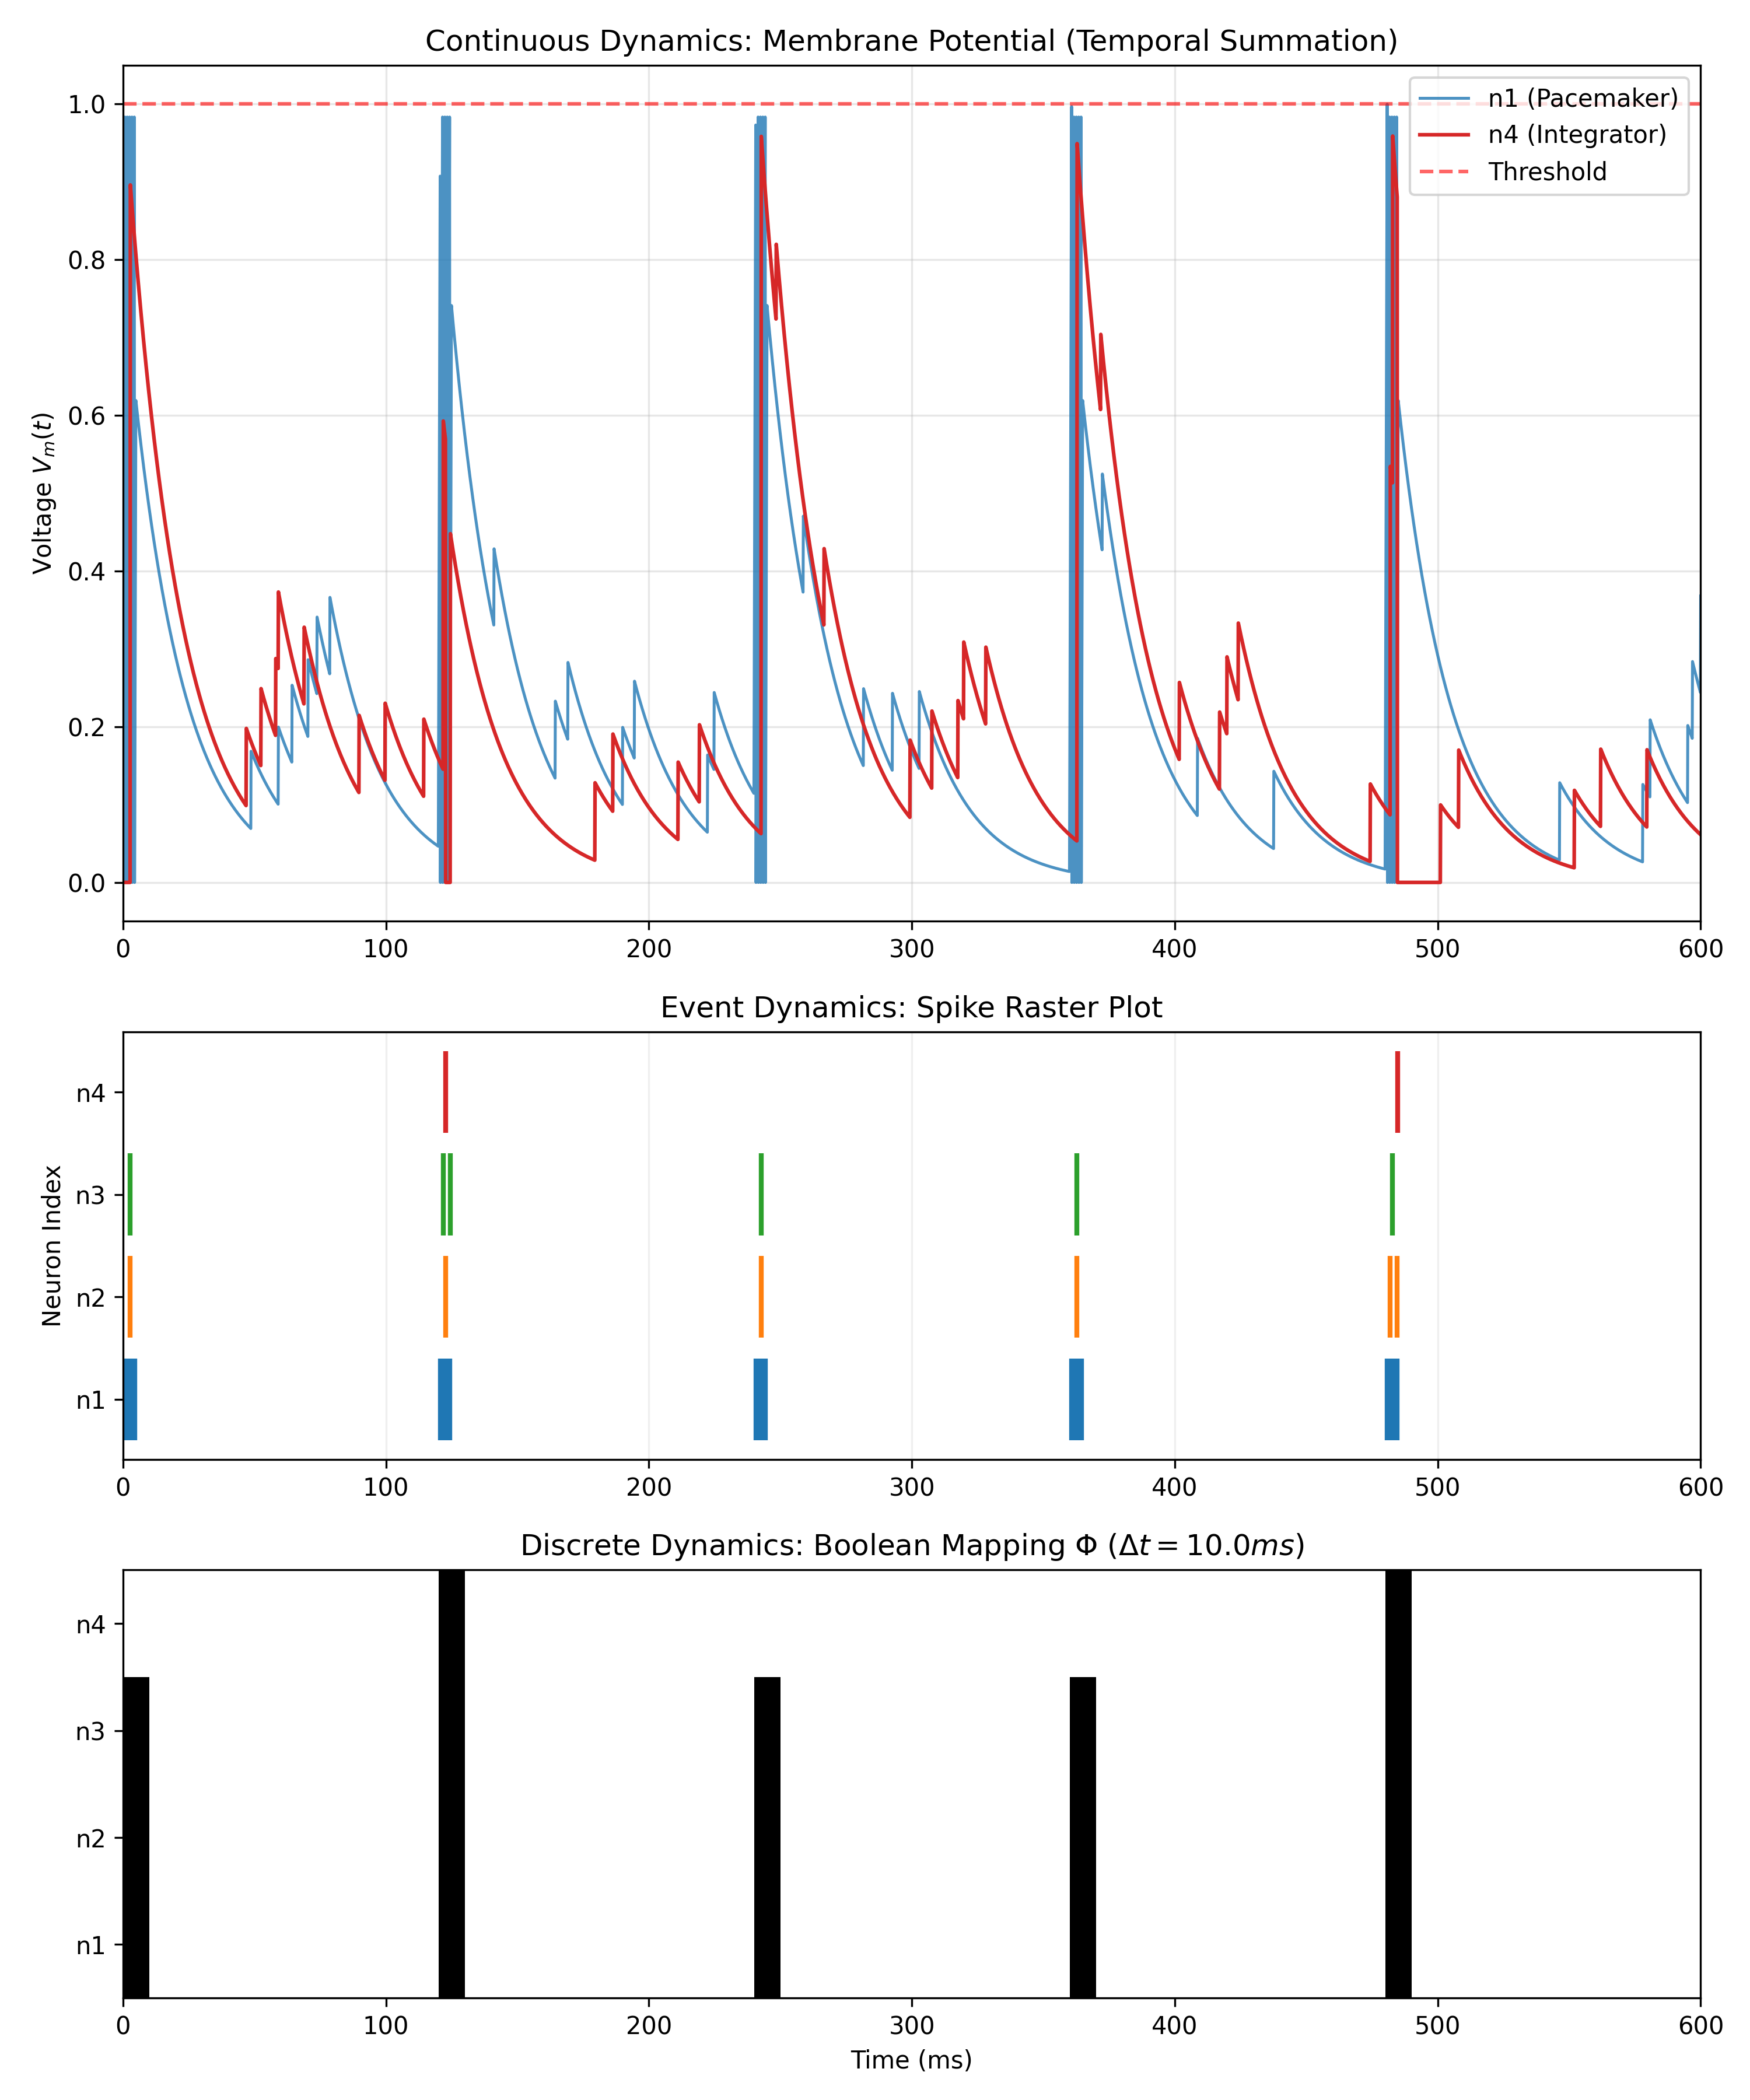
\includegraphics[width=\linewidth]{../results/diamond_validation.png}
    \caption{Mapping of neural dynamics. (Top) Raster plot showing the spiking activity of the four-node network in the continuous LIF domain. (Bottom) Discrete state space representation after applying the $\Phi_{\Delta t}$ operator.}
    \label{fig:validation}
\end{figure}

As shown in Fig. \ref{fig:validation}, the Pacemaker ($n_1$) generates a periodic pulse train. The Relay units ($n_2, n_3$) successfully track these events. Crucially, the Integrator unit ($n_4$) only transitions to state $x_{4}=1$ in the Boolean domain when the spike times of $n_2$ and $n_3$ fall within the same $\Delta t$ interval.

The results confirm that the $\Phi_{\Delta t}$ operator effectively acts as a \textit{coincidence filter}. When the temporal jitter between the relays exceeds $\Delta t$, the integrator remains in a quiescent Boolean state ($0$), demonstrating that the CBN captures the synchronization manifold of the underlying LIF units without the need for continuous integration during the logic phase.

\begin{figure}[h]
    \centering
    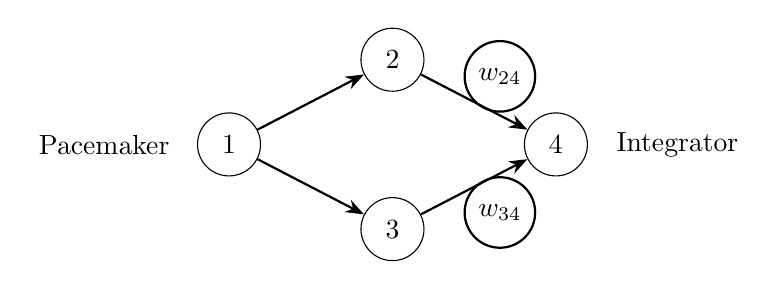
\begin{tikzpicture}[node distance=1.5cm, every node/.style={draw, circle, minimum size=0.8cm}]
        \node (n1) {1};
        \node (n2) [above right=0.5cm and 1.5cm of n1] {2};
        \node (n3) [below right=0.5cm and 1.5cm of n1] {3};
        \node (n4) [below right=0.5cm and 1.5cm of n2] {4};
        
        \draw[->, >=Stealth, thick] (n1) -- (n2);
        \draw[->, >=Stealth, thick] (n1) -- (n3);
        \draw[->, >=Stealth, thick] (n2) -- (n4) node[midway, above right] {$w_{24}$};
        \draw[->, >=Stealth, thick] (n3) -- (n4) node[midway, below right] {$w_{34}$};
        
        \node[draw=none, left=0.2cm of n1] {Pacemaker};
        \node[draw=none, right=0.2cm of n4] {Integrator};
    \end{tikzpicture}
    \caption{Diamond Topology used for coincidence detection validation. The threshold $K_4=2$ ensures $n_4$ only fires when $n_2$ and $n_3$ are synchronized.}
\end{figure}

\subsection{Stochastic Robustness and Poisson Noise}

A critical finding in our validation was the system's resilience to stochastic perturbations. In biological systems, neurons are subject to constant synaptic bombardment, often modeled as a Poisson process. We replaced the standard Gaussian white noise with a Poisson-distributed input:
\begin{equation}
    P(n \text{ spikes in } \Delta t) = \frac{(\lambda \Delta t)^n e^{-\lambda \Delta t}}{n!}
\end{equation}
where $\lambda$ represents the background firing rate. 

As observed in our simulations, the integrator node $n_4$ maintains its logical consistency even when the membrane potentials of $n_2$ and $n_3$ exhibit "jitter" due to Poisson fluctuations. This suggests that the $\Phi_{\Delta t}$ operator acts as a \textit{denoising filter}, extracting the causal logical structure from the underlying noisy biophysical substrate. This finding is crucial for our proposed "Aging Brain" model, as it allows us to distinguish between functional signal degradation and inherent biological noise.

\subsection{Sensitivity Analysis of the Discretization Window $\Delta t$}

The selection of the temporal window $\Delta t$ for the $\Phi_{\Delta t}$ operator is a critical hyperparameter that governs the fidelity of the Boolean mapping. To evaluate its impact, we performed a sensitivity analysis by varying $\Delta t$ between $2ms$ and $50ms$. 

We identify two critical regimes that bound the effectiveness of the discrete mapping:

\begin{enumerate}
    \item \textbf{The Under-sampling Regime ($\Delta t < \tau_m/10$):} When the window is excessively small (e.g., $2ms$), the operator becomes hyper-sensitive to the stochastic fluctuations of the Poisson noise. In this regime, the Boolean state $x_i$ exhibits high-frequency toggling that does not represent functional spiking activity, leading to "logical aliasing." This effectively violates the Nyquist-Shannon sampling theorem, as the discretization frequency exceeds the characteristic integration time of the LIF membrane potential.
    
    \item \textbf{The Saturation Regime ($\Delta t > T_{cycle}$):} Conversely, when $\Delta t$ is too large (e.g., $50ms$), multiple spiking events are collapsed into a single Boolean "1". This leads to a loss of causal resolution, where the coincidence detection in node $n_4$ becomes indistinguishable from independent firing. The network loses its ability to represent the fine-grained temporal summation that characterizes the Diamond topology.
\end{enumerate}

Our results indicate that an optimal window $\Delta t \approx 10-15ms$—approximately half the membrane time constant $\tau_m$—provides the most robust balance. In this "sweet spot," the $\Phi_{\Delta t}$ operator effectively filters sub-threshold Poisson noise while preserving the causal link between the relay nodes ($n_2, n_3$) and the integrator ($n_4$).

%%%%%%%%%%%%%%%%%%%%%%%%%%%%%%%%%%%%%%%%%%%%%%%%%%%%%%%%%%%%%%%%%%%%%%%%

\section{Computational Implementation}

The proposed framework was developed using a vectorized approach in Python 3.12, leveraging the NumPy library for efficient differential equation integration. The simulation environment was deployed on a Linux-based High-Performance Computing (HPC) setup within the Windows Subsystem for Linux (WSL 2) to ensure reproducibility.

One of the most significant findings in this implementation is the reduction in memory footprint. While the LIF simulation requires storing high-precision floating-point arrays for membrane potentials at $0.1ms$ resolution, the resulting CBN state requires only $1$ bit per node per $15ms$. This represents a data compression factor of approximately $150\times$, facilitating the exploration of global attractor landscapes in networks with thousands of entities, a task that remains computationally prohibitive for full biophysical models.

%%%%%%%%%%%%%%%%%%%%%%%%%%%%%%%%%%%%%%%%%%%%%%%%%%%%%%%%%%%%%%%%%%%%%%%%

\section{Conclusions and Future Work}

The $\Phi_{\Delta t}$ operator introduced in this paper provides a rigorous mathematical bridge between the continuous dynamics of the LIF model and the discrete logic of Coupled Boolean Networks. This ``seed'' architecture allows for the study of large-scale neural stability through attractor field analysis while maintaining a direct causal link to the biophysical reality of neuronal spiking. Our validation through the coincidence-detection experiment confirms that the operator effectively preserves functional synchronization properties while significantly reducing computational overhead.

As part of our future research agenda, we plan to explore the following directions:
\begin{itemize}
    \item \textbf{The Criticality Hypothesis:} Investigate how the $\Phi_{\Delta t}$ mapping behaves at the "edge of chaos". We aim to quantify if bio-inspired CBNs naturally gravitate towards critical regimes to maximize information processing.
    \item \textbf{Modeling the Aging Brain:} Use this framework to study neurodegeneration. Specifically, we will test the hypothesis that age-related degradation in synaptic connectivity---modeled as a reduction in $K_a$ or network density---shifts the system from a critical, flexible regime toward an over-ordered, rigid state characterized by reduced transient stability.
    \item \textbf{Large-scale HPC Simulations:} Leverage the efficiency of the CBN formalism to simulate human-scale connectomes, mapping the global attractor landscape derived from empirical EEG and fMRI data.
\end{itemize}

\bibliographystyle{ieeetr}
\bibliography{references}
\end{document}
